\subsubsection{Proton}

Figure\ref{fig:Proton_Event_Display} shows typical EventDisplay of Proton.
Proton has simple structure of events, that is,
as Proton doesn't decay any particles, so it is easy to define stopped point.\\
First, We define `max channel` and `max charge channel` event by event
(then,required single cluster for single event).
`Max channnel` is the channel number of hit which has the most large channel number in the cluster,
and `max charge channel' is the channel number of hit which has the most large amount of signal.
We select events in either following two situations, and define `max channel` as stopped point.

\begin{itemize}
\item max channel $=$ max charge channel \\
\item max channel $=$ max charge channel $+$ 1\\
\end{itemize}

\begin{figure}[htbp]
  \centering
  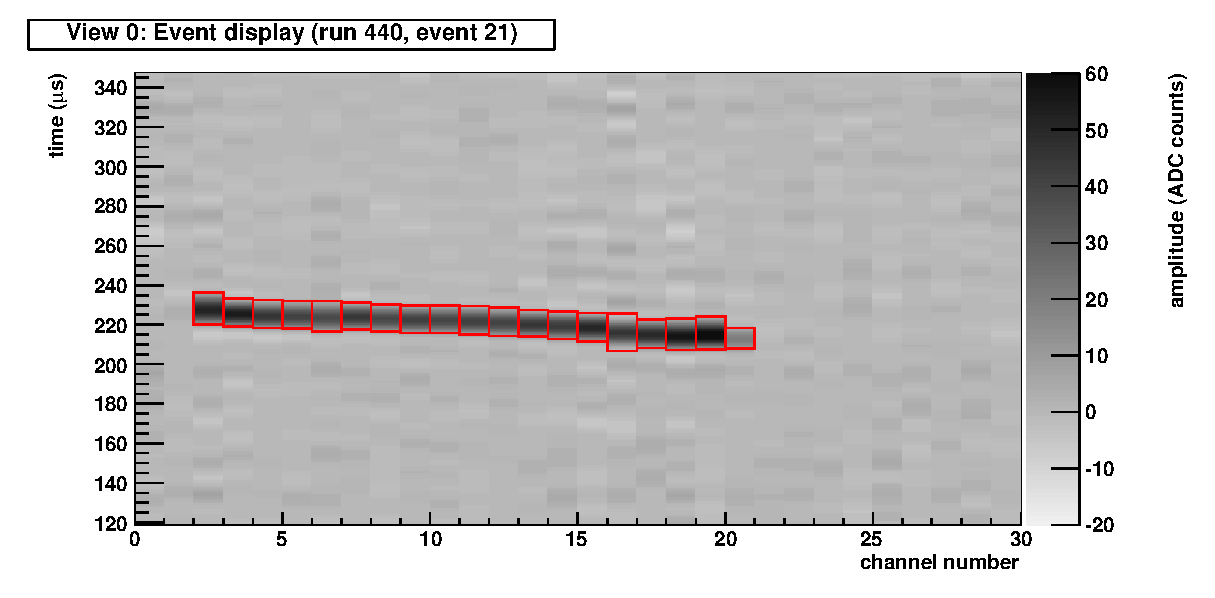
\includegraphics[width=10cm,clip]{./fig/Display_run440_ev21.eps}
  \caption{Typical Event Display of Proton}
  \label{fig:Proton_Event_Display}
\end{figure}
